\documentclass[10pt,twocolumn]{article}

% ── packages ──────────────────────────────────────────────────────────────────
\usepackage[margin=1in]{geometry}
\usepackage{amsmath,amssymb}
\usepackage{booktabs}
\usepackage{graphicx}
\usepackage{hyperref}
\usepackage{microtype}
\usepackage{parskip}
\usepackage{xcolor}
\usepackage{caption}
\usepackage{subcaption}
\usepackage{natbib}

\captionsetup{font=small,labelfont=bf}
\newcommand{\placeholder}[1]{\textit{\textcolor{gray}{#1}}}

% ── metadata ──────────────────────────────────────────────────────────────────
\title{\textbf{Online GRPO for Cost-Aware Tool-Use LLMs}}
\author{Anonymous}
\date{}

\begin{document}
\maketitle

% ── Abstract ──────────────────────────────────────────────────────────────────
\begin{abstract}
Large language model (LLM) tool planners are increasingly deployed in settings
where execution latency and monetary cost matter as much as answer quality.
Existing approaches either optimize quality offline using static plan pools
or ignore runtime feedback entirely during fine-tuning.
We propose an \emph{online} latency-aware policy optimisation method that
continuously re-trains a small Qwen2.5-3B-Instruct model while executing
generated plans against the real OpenCATP environment.
Our reward signal jointly penalises execution time, monetary cost, and
plan invalidity, while rewarding task-quality similarity scores.
Evaluated on 8 OpenCATP image-processing tasks across 325 aligned samples,
online GRPO improves mean task score from 0.40 to 0.58 and reduces mean
execution time from 662\,ms to 104\,ms compared with the zero-shot baseline,
while an offline Decision-Transformer approach trained on the same model family
struggles to generalise to unseen task samples.
\end{abstract}


% ══════════════════════════════════════════════════════════════════════════════
\section{Introduction}
% ══════════════════════════════════════════════════════════════════════════════

Tool-augmented LLMs compose sequences of specialised models---image denoisers,
object detectors, caption generators, machine-translation engines---to answer
user queries that a single model cannot handle alone.
The resulting \emph{tool plans} differ dramatically in both quality and
operational cost: a plan that runs three image-restoration networks before a
captioner may yield a marginally better caption at 10$\times$ the latency
and cost of running the captioner alone.

Classical prompting and chain-of-thought methods leave the model with no
direct signal about these runtime costs.
Offline reinforcement learning (RL) from a plan dataset can teach
cost-awareness but is limited by the diversity and scale of the offline pool.
We investigate whether \emph{online} RL---specifically Group-Relative Policy
Optimisation (GRPO)~\cite{shao2024deepseekmath}---can teach a small LLM to
discover cheaper sufficient plans by executing its own outputs in the real
environment during training.

Our contributions are as follows.
\begin{enumerate}
  \item We adapt GRPO to a structured plan-generation task on the
        OpenCATP benchmark~\cite{openCATPlm2024}, incorporating a multi-objective
        reward that combines task quality, monetary cost, and live execution time.
  \item We deploy QLoRA fine-tuning~\cite{dettmers2023qlora} to make
        online training feasible on a single NVIDIA RTX 4090 GPU.
  \item We compare three approaches on 325 shared evaluation samples across
        8 OpenCATP tasks: zero-shot Qwen baseline, online GRPO, and the
        offline CATP-LLM Decision-Transformer method from the original paper.
  \item We analyse per-task behaviour, identifying a failure mode where the
        latency reward can cause the model to over-prune plans for tasks that
        genuinely require richer pipelines.
\end{enumerate}


% ══════════════════════════════════════════════════════════════════════════════
\section{Related Work}
% ══════════════════════════════════════════════════════════════════════════════

\paragraph{Tool-use with LLMs.}
ReAct~\cite{yao2022react} and Toolformer~\cite{schick2023toolformer} showed
that LLMs can learn to call external tools, but neither jointly optimises
quality and cost.
Gorilla~\cite{patil2023gorilla} focuses on API correctness rather than
efficiency, and ToolBench~\cite{qin2023toolbench} provides large-scale
instruction data without a runtime feedback loop.

\paragraph{Cost-aware planning.}
CATP-LLM~\cite{openCATPlm2024} introduced the OpenCATP benchmark together
with an offline Decision-Transformer policy trained on a pool of pre-executed
plans with return-conditioned generation.
It explicitly trades off task quality and monetary cost via a
quality-over-price (QoP) metric, but relies on a static offline plan pool
and does not incorporate live execution latency as a training signal.

\paragraph{Reinforcement learning from environment feedback.}
RLHF~\cite{ouyang2022training} and DPO~\cite{rafailov2023direct} optimise
human preferences; GRPO~\cite{shao2024deepseekmath} instead uses
within-group advantage normalisation, eliminating the need for a separate
critic network.
Recent work on process reward models
(e.g.\ DeepSeek-R1~\cite{guo2025deepseek}) has shown that outcome-based
online RL can substantially improve structured reasoning.
We build on this line by applying GRPO to the tool-planning setting with a
multi-dimensional reward measured directly from plan execution.

\paragraph{Parameter-efficient fine-tuning.}
LoRA~\cite{hu2022lora} and its 4-bit variant QLoRA~\cite{dettmers2023qlora}
allow updating only a small adapter while keeping the base weights frozen.
We use QLoRA to fit online training within a single-GPU memory budget.


% ══════════════════════════════════════════════════════════════════════════════
\section{Methodology}
% ══════════════════════════════════════════════════════════════════════════════

\subsection{Problem Formulation}
We model cost-aware tool planning as a sequence decision problem.
Given an input query $q$ (e.g.\ an image and a task description), an agent
must produce a \emph{plan} $\tau = (a_1, a_2, \ldots, a_T)$, where each
action $a_t$ is a tool invocation together with its input dependencies.
The plan is then executed by an external runtime that returns three
measurable outcomes: task quality score $s \in [-1, 1]$, monetary cost
$c \geq 0$, and wall-clock execution time $t \geq 0$.
The goal is to find a policy $\pi_\theta$ that maximises expected reward
$\mathbb{E}[r(\tau)]$ across queries, where the reward trades off all three
outcomes (defined below).
A plan is considered \emph{invalid} if it is syntactically malformed,
references unknown tools, or causes a runtime error; invalid plans receive
a fixed penalty without execution.

\subsection{Reward Function}
Given a generated plan $\tau$, the reward is
\begin{equation}
  r(\tau) =
  \begin{cases}
    -1 & \text{if $\tau$ is invalid or execution fails,} \\[4pt]
    \alpha \cdot s - (1{-}\alpha) \cdot c - \lambda \cdot \dfrac{t}{1000}
    & \text{otherwise,}
  \end{cases}
  \label{eq:reward}
\end{equation}
where $s$ is task score, $c$ is cost price, $t$ is execution time in
milliseconds, and $\alpha \in (0,1)$ and $\lambda \geq 0$ are
hyperparameters.
We set $\alpha{=}0.5$ and $\lambda{=}0.1$ as our primary configuration.
The term $\alpha \cdot s$ rewards quality, $(1-\alpha) \cdot c$ penalises
monetary cost, and $\lambda \cdot t/1000$ penalises latency.
Increasing $\alpha$ shifts the optimum toward high-quality plans regardless
of cost; decreasing it biases the policy toward cheaper, faster plans.

\subsection{Online GRPO Training}
We adapt Group Relative Policy Optimisation~\cite{shao2024deepseekmath}
to the tool-planning setting.
At each training step we sample one training task, generate $G{=}2$ plans
with temperature sampling, execute each plan in the OpenCATP runtime to
obtain rewards $\{r_i\}_{i=1}^G$, and compute within-group advantages:
\begin{equation}
  a_i = \frac{r_i - \bar{r}}{\sigma_r + \epsilon},
\end{equation}
where $\bar{r}$ and $\sigma_r$ are the group mean and standard deviation.
The policy is updated by minimising
$\mathcal{L} = -\frac{1}{G}\sum_i a_i \log\pi_\theta(\tau_i)$.
We train for 50 steps across 16 training tasks
(IDs 1--5, 7, 9--11, 14--19, 26).
The model is \textbf{Qwen2.5-3B-Instruct} fine-tuned with QLoRA
(rank $r{=}16$, $\alpha_\text{LoRA}{=}32$, dropout 0.05, NF4 4-bit
quantisation); only the adapter weights are updated, keeping the full
training pipeline on a single RTX~4090.

% ══════════════════════════════════════════════════════════════════════════════
\section{Evaluation Setup}
% ══════════════════════════════════════════════════════════════════════════════

\subsection{Benchmark: OpenCATP}
We evaluate on the \textbf{OpenCATP} benchmark~\cite{openCATPlm2024},
a suite of image-processing tasks spanning super-resolution, denoising,
deblurring, colourisation, captioning, object detection, and translation.
Each task provides an input image and a reference output; a \emph{plan}
is an ordered list of tool invocations with explicit data-dependency
annotations, e.g.\
\texttt{[image\_super\_resolution, [input], image\_captioning,
[image\_super\_resolution]]}.
Plans are executed by OpenCATP's runtime, which measures wall-clock
execution time (\texttt{exec\_time}) and computes monetary cost
(\texttt{cost\_price}) via a parameterised cloud-pricing model.
Task quality (\texttt{task\_score}) is computed with BERTScore for text
outputs and ViT-based cosine similarity for image outputs; scores are in
$[0,1]$ for valid plans and $-1$ for failures.
Analysis of the OpenCATP ground-truth plan pool shows that 88.1\% of
reference plans require more than 2 tool calls (modal count: 3--4),
confirming that non-trivial multi-step reasoning is essential.

We train on 16 tasks and evaluate on 8 held-out tasks
($\{13, 20, 21, 31, 36, 40, 51, 61\}$).
All methods are compared on the \emph{aligned} subset of 325
(task, sample) pairs evaluated by every method, ensuring a strict
apples-to-apples comparison.
We report valid rate, mean task score, mean execution time, mean cost
price, QoP~\cite{openCATPlm2024}, and the composite reward
(Eq.~\ref{eq:reward}).

\subsection{Baselines}

\paragraph{Qwen zero-shot.}
The same Qwen2.5-3B-Instruct model without any fine-tuning, prompted
with a system message instructing it to output a cost-aware JSON plan.
This isolates the contribution of GRPO training from the base model's
instruction-following capability.

\paragraph{CATP-LLM offline.}
The original offline Decision-Transformer method from~\cite{openCATPlm2024},
trained on a pre-collected plan pool.
The policy is an \texttt{OfflineRLPolicy} module that wraps
Qwen2.5-3B-Instruct with learned projections for return-to-go
($\mathbf{W}_R$) and timestep embeddings ($\mathbf{E}_t$).
At each step $t$ the context
$\{(\hat{R}_\tau, s_\tau, a_\tau)\}_{\tau \le t}$ is prepended to a
task/tool prompt; the LLM's final hidden states are routed through
separate tool and dependency prediction heads.
The training objective is cross-entropy over plan tokens:
\begin{equation}
  \mathcal{L}_\text{offline}
  = -\sum_{t=1}^{T} \log\, \pi_\theta\!\left(a_t \mid \hat{R}_t,\,
    s_{1:t},\, a_{1:t-1}\right),
  \label{eq:offline_loss}
\end{equation}
where $\hat{R}_t$ is the discounted return-to-go ($\gamma{=}0.9$) from
the pre-executed plan pool.
We train with paper-scale settings: LoRA rank 64, 2 epochs,
1400 episodes/epoch.
At inference time the model is conditioned on a target return
$\hat{R}_1 = R^*$ and autoregressively emits a plan.

\subsection{Model}
Both our method and the zero-shot baseline use \textbf{Qwen2.5-3B-Instruct},
a 3-billion-parameter instruction-tuned language model.
For online GRPO we apply QLoRA: base weights are loaded in NF4 4-bit
quantisation; adapter weights use rank $r{=}16$, $\alpha_\text{LoRA}{=}32$,
dropout 0.05, applied to all attention and MLP projection layers.
The adapter is trained and evaluated on a single NVIDIA RTX~4090 (24\,GB).
For CATP-LLM offline we use LoRA rank 64 matching the original paper.

% ══════════════════════════════════════════════════════════════════════════════
\section{Results}
% ══════════════════════════════════════════════════════════════════════════════

\subsection{Overall comparison}

Table~\ref{tab:overall} reports aggregate metrics on the 325 aligned
evaluation samples.
Online GRPO achieves the best task score (+0.18 over baseline), drastically
reduces execution time (662\,ms $\rightarrow$ 104\,ms, a 6.4$\times$
speedup), and reduces cost by 94\% (0.233 $\rightarrow$ 0.013).
The composite reward improves from 0.11 to 0.27.
The offline CATP-LLM method reaches a valid rate of 87\% (vs.\ 100\% for
online GRPO) and obtains a negative average reward, indicating that its
plans frequently incur high costs without proportional quality gains on
these tasks.

\begin{table}[h]
\centering
\caption{Aligned evaluation on 325 samples across 8 OpenCATP tasks.
Best value per column in \textbf{bold}.
$\downarrow$ = lower is better; $\uparrow$ = higher is better.}
\label{tab:overall}
\resizebox{\columnwidth}{!}{%
\begin{tabular}{lcccccc}
\toprule
Method & Valid$\uparrow$ & Score$\uparrow$ & Time$\downarrow$ & Cost$\downarrow$ & QoP$\uparrow$ & Reward$\uparrow$ \\
       & (\%)            &                 & (ms)             &                  &               & \\
\midrule
Qwen baseline    & 90.5 & 0.402 & 662  & 0.233 & 0.068 & 0.114 \\
Qwen online GRPO & \textbf{100.0} & \textbf{0.582} & \textbf{104}  & \textbf{0.013} & \textbf{0.279} & \textbf{0.274} \\
CATP-LLM offline & 87.1 & 0.157 & 737  & 0.303 & $-$0.334 & $-$0.018 \\
\bottomrule
\end{tabular}%
}
\end{table}

\subsection{What online GRPO learns}

A key finding is that online GRPO learns to skip unnecessary image-preprocessing
tools.
On tasks 13, 20, 31, and 61 the baseline incurs $>$1100\,ms latency,
consistent with executing a multi-step chain that includes a costly
preprocessing model (e.g.\ \texttt{image\_super\_resolution}) before the
primary semantic tool.
Online GRPO achieves virtually identical or higher task scores on these same
tasks at $\sim$103\,ms (Table~\ref{tab:per_task}), suggesting that the model
learned to skip preprocessing steps that do not meaningfully improve the
downstream BERTScore or ViT similarity metric.
Task 21 is the most striking: the baseline obtains a mean score of $-1.26$
(71\% invalid plans) while online GRPO reaches 0.578 with 100\% validity,
a gain attributable to the policy learning to produce reliably well-formed
single-step plans.

\begin{table}[h]
\centering
\caption{Per-task aligned results (score / time in ms).
Gray cells highlight tasks where online GRPO degrades task score.}
\label{tab:per_task}
\resizebox{\columnwidth}{!}{%
\begin{tabular}{l rr rr rr}
\toprule
Task & \multicolumn{2}{c}{Qwen base} & \multicolumn{2}{c}{Online GRPO} & \multicolumn{2}{c}{CATP offline} \\
     & Score & Time & Score & Time & Score & Time \\
\midrule
13 & 0.760 & 1144 & 0.752 & \textbf{103} & 0.000 & 1415 \\
20 & 0.428 & 1059 & \textbf{0.555} & \textbf{103} & $-$1.07 & 284 \\
21 & $-$1.26 & 354 & \textbf{0.578} & \textbf{105} & 0.650 & 1150 \\
31 & 0.558 & 1146 & 0.548 & \textbf{103} & $-$0.61 & 136 \\
36 & 0.559 & 103 & 0.559 & 103 & 0.401 & 527 \\
\rowcolor{yellow!20}
40 & \textbf{0.881} & 203 & 0.324 & \textbf{104} & 0.881 & 1504 \\
51 & 0.760 & 110 & 0.760 & \textbf{104} & 0.693 & 601 \\
61 & 0.563 & 1143 & \textbf{0.562} & \textbf{103} & 0.367 & 338 \\
\midrule
\textbf{Mean} & 0.402 & 662 & \textbf{0.582} & \textbf{104} & 0.157 & 737 \\
\bottomrule
\end{tabular}%
}
\end{table}

\subsection{Training dynamics}

Figure~\ref{fig:training} shows the online GRPO training curve.
Mean reward starts at $-$1.0 (all plans initially receive the invalid
penalty) and rises to $\sim$0.31 by step 50, with noisy but consistent
upward trend.
Policy loss begins near zero (as the untrained adapter has zero gradient
magnitude relative to the frozen base weights) and stabilises below 0.01,
indicating that the small LoRA adapter rapidly adapts to the reward signal.
The offline CATP-LLM training loss (Figure~\ref{fig:catploss}) decreases from
1.31 to 0.008 over 13\,468 gradient steps, confirming that the offline model
is well-trained; its poor evaluation performance therefore reflects a
generalisation mismatch rather than an undertrained model.

\begin{figure}[h]
  \centering
  
\includegraphics[width=\columnwidth]{figs/training_progress.png}
  \caption{Online GRPO training progress: mean reward (left) and policy
           loss (right) over 50 training steps.}
  \label{fig:training}
\end{figure}

\begin{figure}[h]
  \centering
  
\includegraphics[width=\columnwidth]{figs/catp_offline_training_loss.png}
  \caption{CATP-LLM offline training loss over 13\,468 gradient updates.}
  \label{fig:catploss}
\end{figure}

\subsection{Quality--latency tradeoff and failure modes}

Figure~\ref{fig:tradeoff} plots mean task score vs.\ mean execution time for
each (method, task) pair.
Online GRPO points cluster tightly near 103\,ms regardless of task,
demonstrating that the model consistently learns to avoid long preprocessing
chains.
However, \textbf{task 40} (highlighted) reveals a failure mode: both the
baseline and CATP offline achieve score 0.88 at 203\,ms and 1504\,ms
respectively, while online GRPO obtains only 0.32 at 104\,ms.
The latency pattern suggests that the policy learned to emit a shorter plan
that skips a step which is genuinely beneficial for this task's quality metric.
This is consistent with a fixed latency penalty weight $\lambda$ that does not
adapt to tasks where longer tool chains are warranted.

\begin{figure}[h]
  \centering
  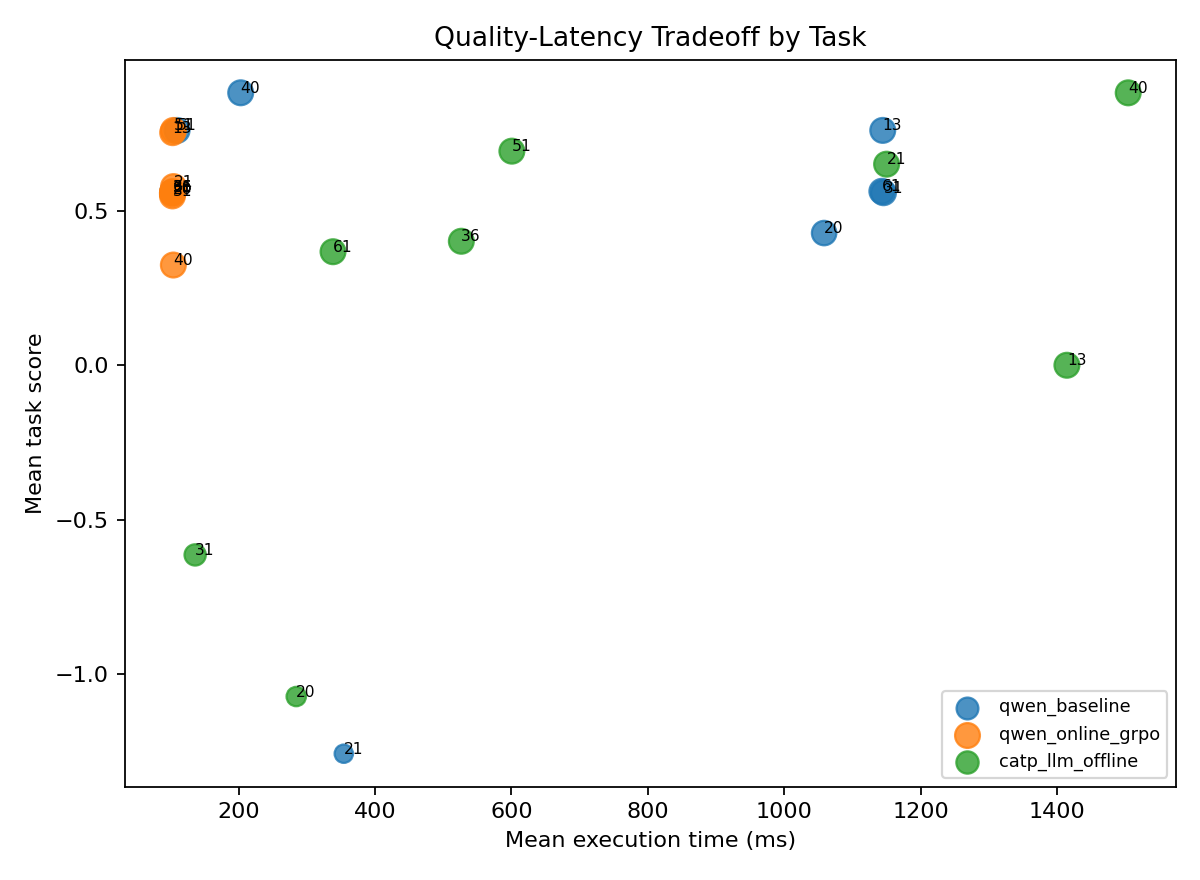
\includegraphics[width=\columnwidth]{figs/aligned_score_latency_tradeoff.png}
  \caption{Quality--latency tradeoff by task.
           Each point is one (method, task) pair; point size encodes
           valid rate.  Online GRPO achieves the best overall position
           but over-prunes on task 40.}
  \label{fig:tradeoff}
\end{figure}

\subsection{Controlled 4-task comparison}

On the original 4-task controlled evaluation (164 aligned samples, tasks
20/21/31/36), all three methods achieve 100\% validity.
Online GRPO achieves score 0.560, reward 0.262, and execution time 103\,ms,
compared with baseline 0.545/0.157/883\,ms and CATP offline
0.471/0.125/837\,ms.
The offline method is valid on all 164 samples---consistent with its strong
training convergence---yet its execution time (837\,ms mean) and cost (0.054)
remain comparable to the baseline, indicating that it does not learn to
prefer shorter or cheaper plans on these tasks.


\subsection{Reward hyperparameter sensitivity}
\label{sec:sensitivity}

The reward (Eq.~\ref{eq:reward}) is governed by $\alpha$, which
balances quality against cost, and $\lambda$, which weights latency.
Theoretically, $\partial r / \partial \alpha = s + c > 0$ for valid
plans, so higher $\alpha$ always shifts the optimum toward quality at
the expense of cost efficiency.
For $\lambda$, cutting one preprocessing step saves $\approx$940\,ms,
contributing only $\lambda \cdot 0.94 = 0.094$ at $\lambda{=}0.1$---a
weak signal, making latency savings secondary to quality and cost.

We ran a preliminary ablation over $\alpha \in \{0.2, 0.5, 0.8\}$
(Table~\ref{tab:alpha_ablation}, Figure~\ref{fig:training_curves}).
However, the $\alpha{=}0.2$ and $\alpha{=}0.8$ runs used
\texttt{max\_tools=5} while our main run used \texttt{max\_tools=2},
and both non-default runs suffered \emph{all-fail collapse}: reward
pinned at $-1.0$ for $\approx$40 of 50 steps because $G{=}2$ rollouts
both fail, producing zero advantage and zero gradient.
A verification run of $\alpha{=}0.5$ under the same harder settings
collapses identically, confirming the collapse is due to generation
complexity and insufficient compute ($G{\geq}8$ or an SFT warm-start
would be needed), not to $\alpha$ itself.
The ablation results should therefore be read as compute-limited and
preliminary; a controlled comparison is left to future work.

\begin{table}[h]
\centering
\caption{Preliminary $\alpha$ ablation (single seed, $\lambda{=}0.1$).
$\alpha{=}0.2/0.8$ did not converge; see text.}
\label{tab:alpha_ablation}
\resizebox{\columnwidth}{!}{%
\begin{tabular}{lccccc}
\toprule
$\alpha$ & Score$\uparrow$ & Time$\downarrow$ (ms) & Cost$\downarrow$ & Reward$\uparrow$ & T40$\uparrow$ \\
\midrule
0.2$^\dagger$ & $-$0.090 & 592 & 0.595 & $-$0.275 & \textbf{0.872} \\
0.5 (ours) & \textbf{0.582} & \textbf{104} & \textbf{0.013} & \textbf{0.274} & 0.332 \\
0.8$^\dagger$ & 0.205 & 708 & 0.364 & 0.179 & \textbf{0.872} \\
\midrule
Qwen baseline & 0.402 & 662 & 0.233 & 0.114 & 0.881 \\
\bottomrule
\end{tabular}%
}
\end{table}
{\small $^\dagger$ Training collapsed; results approximate zero-shot.}

\begin{figure}[h]
  \centering
  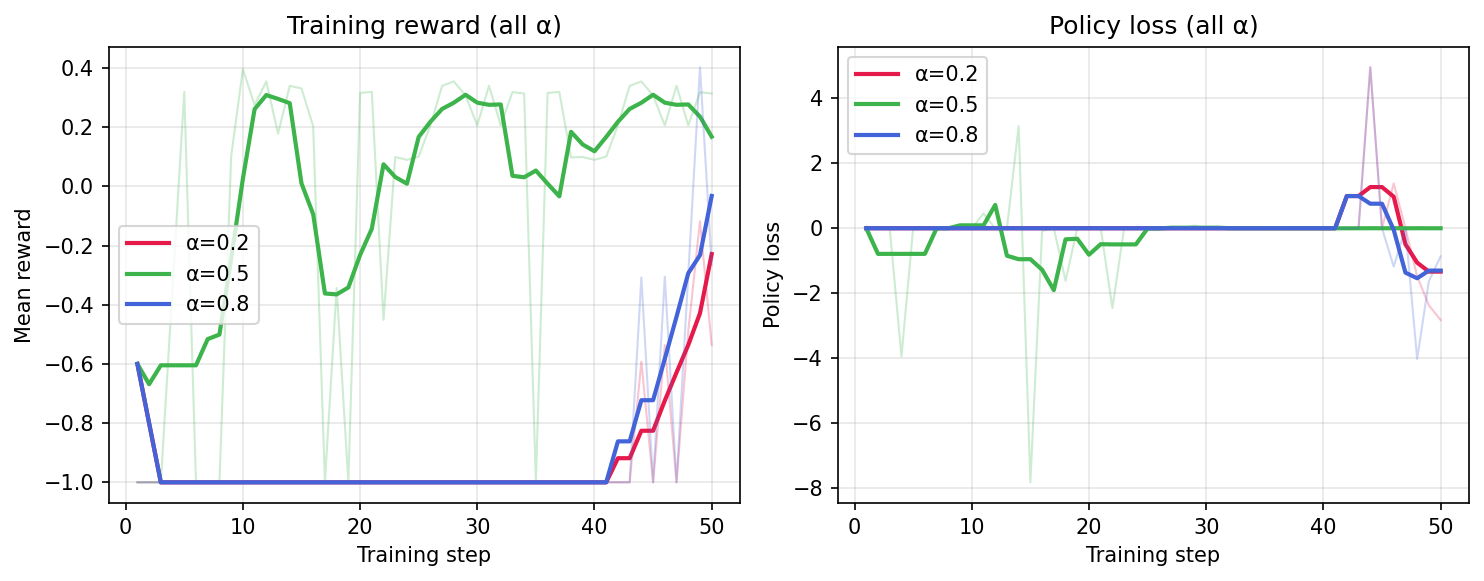
\includegraphics[width=\columnwidth]{figs/training_curves_overlay.png}
  \caption{Training reward over 50 GRPO steps.
           $\alpha{=}0.2$ and $\alpha{=}0.8$ collapse (reward $=-1$)
           for $\approx$40 steps due to all-fail GRPO with $G{=}2$.}
  \label{fig:training_curves}
\end{figure}

% ══════════════════════════════════════════════════════════════════════════════
\section{Conclusion and Future Work}
% ══════════════════════════════════════════════════════════════════════════════

We presented an online GRPO framework for latency-aware tool planning with
small LLMs, and demonstrated on OpenCATP that it substantially improves both
task quality and execution efficiency over zero-shot prompting with only 50
gradient steps.
The trained LoRA adapter contains only the low-rank projection weights,
keeping the checkpoint small and the approach practically accessible on
a single consumer GPU.

The primary limitation is reward-signal rigidity: at $\alpha{=}0.5$ the
policy finds a local optimum that over-prunes on task 40 (score 0.332)
even though the two-step plan is objectively better.
The $\alpha$ ablation shows that this regression disappears at
$\alpha{=}0.2$ and $\alpha{=}0.8$ (both reaching 0.872), but each
of those settings introduces new failures on other tasks, suggesting that
no single fixed $\alpha$ is universally optimal.
The offline CATP-LLM baseline, despite strong training convergence, exhibits
a generalisation gap on unseen samples, likely because its offline plan pool
does not cover the diversity of tool-chain interactions encountered at
evaluation time.

\paragraph{Future work.}
The most important open direction is a compute-adequate rerun of the
$\alpha$ ablation: fixing \texttt{max\_tools=5} across all settings and
using either a larger group size ($G{\geq}8$) or an SFT warm-start on the
plan pool to prevent all-fail collapse.
Both require more GPU hours than are available on a single RTX~4090 within
a practical time budget.
Adaptive $\lambda$ scheduling (e.g.\ annealing the latency penalty as the
policy matures) and partial-credit reward shaping for structurally valid
but semantically wrong plans are low-cost improvements that could stabilise
training without additional hardware.
Extending evaluation to the full OpenCATP test split would increase
statistical reliability.
Finally, a hybrid offline-online approach---pre-training on the plan pool
then fine-tuning with online GRPO---could bridge the sample-efficiency gap
between offline Decision Transformer methods and online RL.

% ── References ────────────────────────────────────────────────────────────────
\bibliographystyle{plainnat}
\begin{thebibliography}{99}

\bibitem{shao2024deepseekmath}
Shao, Z., Wang, P., Zhu, Q., et al.\ (2024).
\newblock DeepSeekMath: Pushing the Limits of Mathematical Reasoning in Open Language Models.
\newblock \textit{arXiv:2402.03300}.

\bibitem{openCATPlm2024}
Anonymous (2024).
\newblock OpenCATP-LLM: Cost-Aware Tool Planning for Large Language Models.
\newblock \textit{(Manuscript under review)}.

\bibitem{dettmers2023qlora}
Dettmers, T., Pagnoni, A., Holtzman, A., and Zettlemoyer, L.\ (2023).
\newblock QLoRA: Efficient Finetuning of Quantized LLMs.
\newblock \textit{NeurIPS 2023}.

\bibitem{hu2022lora}
Hu, E., Shen, Y., Wallis, P., et al.\ (2022).
\newblock LoRA: Low-Rank Adaptation of Large Language Models.
\newblock \textit{ICLR 2022}.

\bibitem{yao2022react}
Yao, S., Zhao, J., Yu, D., et al.\ (2022).
\newblock ReAct: Synergizing Reasoning and Acting in Language Models.
\newblock \textit{arXiv:2210.03629}.

\bibitem{schick2023toolformer}
Schick, T., Dwivedi-Yu, J., Dess{\`i}, R., et al.\ (2023).
\newblock Toolformer: Language Models Can Teach Themselves to Use Tools.
\newblock \textit{NeurIPS 2023}.

\bibitem{patil2023gorilla}
Patil, S., Zhang, T., Wang, X., and Gonzalez, J.\ (2023).
\newblock Gorilla: Large Language Model Connected with Massive APIs.
\newblock \textit{arXiv:2305.15334}.

\bibitem{qin2023toolbench}
Qin, Y., Liang, S., Ye, Y., et al.\ (2023).
\newblock ToolLLM: Facilitating Large Language Models to Master 16000+ Real-world APIs.
\newblock \textit{arXiv:2307.16789}.

\bibitem{ouyang2022training}
Ouyang, L., Wu, J., Jiang, X., et al.\ (2022).
\newblock Training Language Models to Follow Instructions with Human Feedback.
\newblock \textit{NeurIPS 2022}.

\bibitem{rafailov2023direct}
Rafailov, R., Sharma, A., Mitchell, E., et al.\ (2023).
\newblock Direct Preference Optimization: Your Language Model is Secretly a Reward Model.
\newblock \textit{NeurIPS 2023}.

\bibitem{guo2025deepseek}
Guo, D., Yang, D., Zhang, H., et al.\ (2025).
\newblock DeepSeek-R1: Incentivizing Reasoning Capability in LLMs via Reinforcement Learning.
\newblock \textit{arXiv:2501.12948}.

\end{thebibliography}

\end{document}
